%%%%%%%%%%%%%%%%%%%%%%%%%%%%%%%%%%%%%%%%%%%%%%%%%%%%%%%%%%%%%%%
%% BRIEF VERSION OF OXFORD THESIS TEMPLATE FOR CHAPTER PREVIEWS

%%%%% CHOOSE PAGE LAYOUT
% format for PDF output (ie equal margins, no extra blank pages):
\documentclass[a4paper,nobind]{templates/ociamthesis}

% UL 5 January 2021 - add packages used by kableExtra
\usepackage{booktabs}
\usepackage{longtable}
\usepackage{array}
\usepackage{multirow}
\usepackage{wrapfig}
\usepackage{colortbl}
\usepackage{pdflscape}
\usepackage{tabu}
\usepackage{threeparttable}
\usepackage{threeparttablex}
\usepackage[normalem]{ulem}
\usepackage{makecell}
\usepackage[colorlinks=false,pdfpagelabels,hidelinks=]{hyperref}
\usepackage{float}


%UL set section header spacing
\usepackage{titlesec}
% 
\titlespacing\subsubsection{0pt}{24pt plus 4pt minus 2pt}{0pt plus 2pt minus 2pt}

% UL 30 Nov 2018 pandoc puts lists in 'tightlist' command when no space between bullet points in Rmd file
\providecommand{\tightlist}{%
  \setlength{\itemsep}{0pt}\setlength{\parskip}{0pt}}
 
% UL 1 Dec 2018, fix to include code in shaded environments
\usepackage{color}
\usepackage{fancyvrb}
\newcommand{\VerbBar}{|}
\newcommand{\VERB}{\Verb[commandchars=\\\{\}]}
\DefineVerbatimEnvironment{Highlighting}{Verbatim}{commandchars=\\\{\}}
% Add ',fontsize=\small' for more characters per line
\usepackage{framed}
\definecolor{shadecolor}{RGB}{248,248,248}
\newenvironment{Shaded}{\begin{snugshade}}{\end{snugshade}}
\newcommand{\AlertTok}[1]{\textcolor[rgb]{0.94,0.16,0.16}{#1}}
\newcommand{\AnnotationTok}[1]{\textcolor[rgb]{0.56,0.35,0.01}{\textbf{\textit{#1}}}}
\newcommand{\AttributeTok}[1]{\textcolor[rgb]{0.77,0.63,0.00}{#1}}
\newcommand{\BaseNTok}[1]{\textcolor[rgb]{0.00,0.00,0.81}{#1}}
\newcommand{\BuiltInTok}[1]{#1}
\newcommand{\CharTok}[1]{\textcolor[rgb]{0.31,0.60,0.02}{#1}}
\newcommand{\CommentTok}[1]{\textcolor[rgb]{0.56,0.35,0.01}{\textit{#1}}}
\newcommand{\CommentVarTok}[1]{\textcolor[rgb]{0.56,0.35,0.01}{\textbf{\textit{#1}}}}
\newcommand{\ConstantTok}[1]{\textcolor[rgb]{0.00,0.00,0.00}{#1}}
\newcommand{\ControlFlowTok}[1]{\textcolor[rgb]{0.13,0.29,0.53}{\textbf{#1}}}
\newcommand{\DataTypeTok}[1]{\textcolor[rgb]{0.13,0.29,0.53}{#1}}
\newcommand{\DecValTok}[1]{\textcolor[rgb]{0.00,0.00,0.81}{#1}}
\newcommand{\DocumentationTok}[1]{\textcolor[rgb]{0.56,0.35,0.01}{\textbf{\textit{#1}}}}
\newcommand{\ErrorTok}[1]{\textcolor[rgb]{0.64,0.00,0.00}{\textbf{#1}}}
\newcommand{\ExtensionTok}[1]{#1}
\newcommand{\FloatTok}[1]{\textcolor[rgb]{0.00,0.00,0.81}{#1}}
\newcommand{\FunctionTok}[1]{\textcolor[rgb]{0.00,0.00,0.00}{#1}}
\newcommand{\ImportTok}[1]{#1}
\newcommand{\InformationTok}[1]{\textcolor[rgb]{0.56,0.35,0.01}{\textbf{\textit{#1}}}}
\newcommand{\KeywordTok}[1]{\textcolor[rgb]{0.13,0.29,0.53}{\textbf{#1}}}
\newcommand{\NormalTok}[1]{#1}
\newcommand{\OperatorTok}[1]{\textcolor[rgb]{0.81,0.36,0.00}{\textbf{#1}}}
\newcommand{\OtherTok}[1]{\textcolor[rgb]{0.56,0.35,0.01}{#1}}
\newcommand{\PreprocessorTok}[1]{\textcolor[rgb]{0.56,0.35,0.01}{\textit{#1}}}
\newcommand{\RegionMarkerTok}[1]{#1}
\newcommand{\SpecialCharTok}[1]{\textcolor[rgb]{0.00,0.00,0.00}{#1}}
\newcommand{\SpecialStringTok}[1]{\textcolor[rgb]{0.31,0.60,0.02}{#1}}
\newcommand{\StringTok}[1]{\textcolor[rgb]{0.31,0.60,0.02}{#1}}
\newcommand{\VariableTok}[1]{\textcolor[rgb]{0.00,0.00,0.00}{#1}}
\newcommand{\VerbatimStringTok}[1]{\textcolor[rgb]{0.31,0.60,0.02}{#1}}
\newcommand{\WarningTok}[1]{\textcolor[rgb]{0.56,0.35,0.01}{\textbf{\textit{#1}}}}

%UL 2 Dec 2018 add a bit of white space before and after code blocks
\renewenvironment{Shaded}
{
  \vspace{10pt}%
  \begin{snugshade}%
}{%
  \end{snugshade}%
  \vspace{8pt}%
}
%UL 2 Dec 2018 reduce whitespace around verbatim environments
\usepackage{etoolbox}
\makeatletter
\preto{\@verbatim}{\topsep=0pt \partopsep=0pt }
\makeatother

%UL 28 Mar 2019, enable strikethrough
\usepackage[normalem]{ulem}

%UL use soul package for correction highlighting
\usepackage{soul}
\usepackage{xcolor}
\newcommand{\ctext}[3][RGB]{%
  \begingroup
  \definecolor{hlcolor}{#1}{#2}\sethlcolor{hlcolor}%
  \hl{#3}%
  \endgroup
}
\soulregister\ref7
\soulregister\cite7
\soulregister\autocite7
\soulregister\textcite7
\soulregister\pageref7

%UL 3 Nov 2019, avoid mysterious error from not having hyperref included
\usepackage{hyperref}

%%%%% SELECT YOUR DRAFT OPTIONS
% Three options going on here; use in any combination.  But remember to turn the first two off before
% generating a PDF to send to the printer!

% This adds a "DRAFT" footer to every normal page.  (The first page of each chapter is not a "normal" page.)

% This highlights (in blue) corrections marked with (for words) \mccorrect{blah} or (for whole
% paragraphs) \begin{mccorrection} . . . \end{mccorrection}.  This can be useful for sending a PDF of
% your corrected thesis to your examiners for review.  Turn it off, and the blue disappears.

%%%%% BIBLIOGRAPHY SETUP
% Note that your bibliography will require some tweaking depending on your department, preferred format, etc.
% The options included below are just very basic "sciencey" and "humanitiesey" options to get started.
% If you've not used LaTeX before, I recommend reading a little about biblatex/biber and getting started with it.
% If you're already a LaTeX pro and are used to natbib or something, modify as necessary.
% Either way, you'll have to choose and configure an appropriate bibliography format...

% The science-type option: numerical in-text citation with references in order of appearance.
% \usepackage[style=numeric-comp, sorting=none, backend=biber, doi=false, isbn=false]{biblatex}
% \newcommand*{\bibtitle}{References}

% The humanities-type option: author-year in-text citation with an alphabetical works cited.
% \usepackage[style=authoryear, sorting=nyt, backend=biber, maxcitenames=2, useprefix, doi=false, isbn=false]{biblatex}
% \newcommand*{\bibtitle}{Works Cited}

%UL 3 Dec 2018: set this from YAML in index.Rmd
\usepackage[style=numeric-comp, sorting=none, backend=biber, doi=false, isbn=false]{biblatex}
\newcommand*{\bibtitle}{References}

% This makes the bibliography left-aligned (not 'justified') and slightly smaller font.
\renewcommand*{\bibfont}{\raggedright\small}

% Change this to the name of your .bib file (usually exported from a citation manager like Zotero or EndNote).
\addbibresource{references.bib}

%%%%% YOUR OWN PERSONAL MACROS
% This is a good place to dump your own LaTeX macros as they come up.

% To make text superscripts shortcuts
	\renewcommand{\th}{\textsuperscript{th}} % ex: I won 4\th place
	\newcommand{\nd}{\textsuperscript{nd}}
	\renewcommand{\st}{\textsuperscript{st}}
	\newcommand{\rd}{\textsuperscript{rd}}

%%%%% THE ACTUAL DOCUMENT STARTS HERE
\begin{document}

%%%%% CHOOSE YOUR LINE SPACING HERE
% This is the official option.  Use it for your submission copy and library copy:
\setlength{\textbaselineskip}{22pt plus2pt}
% This is closer spacing (about 1.5-spaced) that you might prefer for your personal copies:
%\setlength{\textbaselineskip}{18pt plus2pt minus1pt}

% UL: You can set the general paragraph spacing here - I've set it to 2pt (was 0) so
% it's less claustrophobic
\setlength{\parskip}{2pt plus 1pt}

% Leave this line alone; it gets things started for the real document.
\setlength{\baselineskip}{\textbaselineskip}

% all your chapters and appendices will appear here
\begin{savequote}
Neque porro quisquam est qui dolorem ipsum quia dolor sit amet,
consectetur, adipisci velit\ldots{}

There is no one who loves pain itself, who seeks after it and wants to
have it, simply because it is pain\ldots{}
\end{savequote}



\chapter{R Markdown basics}\label{rmd-basics}

\minitoc <!-- this will include a mini table of contents-->

\noindent Here is a brief introduction to using \emph{R Markdown}.
\emph{Markdown} is a simple formatting syntax for authoring HTML, PDF,
and MS Word documents and much, much more. \emph{R Markdown} provides
the flexibility of \emph{Markdown} with the implementation of \textbf{R}
input and output. For more details on using \emph{R Markdown} see
\url{http://rmarkdown.rstudio.com}.

\section{Basic markdown syntax}\label{basic-markdown-syntax}

\subsection{Whitespace}\label{whitespace}

Be careful with your spacing. While whitespace largely is ignored, it
does at times give markdown signals as to how to proceed. As a habit,
try to keep everything left aligned whenever possible, especially as you
type a new paragraph. In other words, there is no need to indent basic
text in the Rmd document (in fact, it might cause your text to do funny
things if you do).

\subsection{Italics and bold}\label{italics-and-bold}

\begin{itemize}
\tightlist
\item
  \emph{Italics} are done like *this* or \_this\_
\item
  \textbf{Bold} is done like **this** or \_\_this\_\_
\item
  \textbf{\emph{Bold and italics}} is done like ***this***,
  \_\_\_this\_\_\_, or (the most transparent solution, in my opinion)
  **\_this\_**
\end{itemize}

\subsection{Inline code}\label{inline-code}

\begin{itemize}
\tightlist
\item
  \texttt{Inline\ code} is created with backticks like
  \texttt{\textasciigrave{}this\textasciigrave{}}
\end{itemize}

\subsection{Sub and superscript}\label{sub-and-superscript}

Sub\textsubscript{2} and super\textsuperscript{2} script is created like
this\textasciitilde{}2\textasciitilde{} and this\^{}2\^{}

\subsection{Strikethrough}\label{strikethrough}

\begin{itemize}
\tightlist
\item
  \sout{Strikethrough} is done \textasciitilde{}\textasciitilde{}like
  this\textasciitilde{}\textasciitilde{}
\end{itemize}

\subsection{\texorpdfstring{`Escaping' (aka ``What if I need an actual
asterisk?'')}{Escaping (aka What if I need an actual asterisk?)}}\label{escaping-aka-what-if-i-need-an-actual-asterisk}

\begin{itemize}
\tightlist
\item
  To include an actual *, \_ or \textbackslash{}, add another
  \textbackslash{} in front of them: \textbackslash{}*,
  \textbackslash{}\_, \textbackslash{}\textbackslash{}
\end{itemize}

\subsection{Endash (--), emdash (---)}\label{endash-emdash}

\begin{itemize}
\tightlist
\item
  -- and --- with -\/- and -\/-\/-
\end{itemize}

\subsection{Blockquotes}\label{blockquotes}

Do like this:

\begin{quote}
Put a \textgreater{} in front of the line.
\end{quote}

\subsection{Headings}\label{headings}

Section headers are created with \#'s of increasing number, i.e.

\begin{itemize}
\tightlist
\item
  \# First-level heading
\item
  \#\# Second-level heading
\item
  \#\#\# Etc.
\end{itemize}

In PDF output, a level-five heading will turn into a paragraph heading,
i.e. \texttt{\textbackslash{}paragraph\{My\ level-five\ heading\}},
which appears as bold text on the same line as the subsequent paragraph.

\subsection{Lists}\label{lists}

Unordered list by starting a line with an * or a -:

\begin{itemize}
\tightlist
\item
  Item 1
\item
  Item 2
\end{itemize}

Ordered lists by starting a line with a number. Notice that you can
mislabel the numbers and \emph{Markdown} will still make the order right
in the output:

\begin{enumerate}
\def\labelenumi{\arabic{enumi}.}
\tightlist
\item
  Item 1
\item
  Item 2
\end{enumerate}

To create a sublist, indent the values a bit (at least four spaces or a
tab):

\begin{enumerate}
\def\labelenumi{\arabic{enumi}.}
\tightlist
\item
  Item 1
\item
  Item 2
\item
  Item 3

  \begin{itemize}
  \tightlist
  \item
    Item 3a
  \item
    Item 3b
  \end{itemize}
\end{enumerate}

\subsection{Line breaks}\label{line-breaks}

The official \emph{Markdown} way to create line breaks is by ending a
line with more than two spaces.

Roses are red. Violets are blue.

This appears on the same line in the output, because we didn't add
spaces after red.

Roses are red.\\
Violets are blue.

This appears with a line break because I added spaces after red.

I find this is confusing, so I recommend the alternative way: Ending a
line with a backslash will also create a linebreak:

Roses are red.\\
Violets are blue.

To create a new paragraph, you put a blank line.

Therefore, this line starts its own paragraph.

\subsection{Hyperlinks}\label{hyperlinks}

\begin{itemize}
\tightlist
\item
  \href{https://www.google.com}{This is a hyperlink} created by writing
  the text you want turned into a clickable link in
  \texttt{{[}square\ brackets\ followed\ by\ a{]}(https://hyperlink-in-parentheses)}
\end{itemize}

\subsection{Footnotes}\label{footnotes}

\begin{itemize}
\tightlist
\item
  Are created\footnote{my footnote text} by writing either \^{}{[}my
  footnote text{]} for supplying the footnote content inline, or
  something like \texttt{{[}\^{}a-random-footnote-label{]}} and
  supplying the text elsewhere in the format shown below \footnote{This
    is a random test.}:
\end{itemize}

\texttt{{[}\^{}a-random-footnote-label{]}:\ This\ is\ a\ random\ test.}

\subsection{Comments}\label{comments}

To write comments within your text that won't actually be included in
the output, use the same syntax as for writing comments in HTML. That
is, \textless{}!-\/- this will not be included in the output
-\/-\textgreater{}.

\subsection{Math}\label{math}

The syntax for writing math is stolen from LaTeX. To write a math
expression that will be shown \textbf{inline}, enclose it in dollar
signs. - This: \$A = \textbackslash{}pi*r\^{}\{2\}\$ Becomes:
\(A = \pi*r^{2}\)

To write a math expression that will be shown in a block, enclose it in
two dollar signs.\\
This: \$\$A = \textbackslash{}pi*r\^{}\{2\}\$\$

Becomes: \[A = \pi*r^{2}\]

To create numbered equations, put them in an `equation' environment and
give them a label with the syntax \texttt{(\textbackslash{}\#eq:label)},
like this:

\begin{Shaded}
\begin{Highlighting}[]
\KeywordTok{\textbackslash{}begin}\NormalTok{\{}\ExtensionTok{equation}\NormalTok{\}}\SpecialStringTok{ }
\SpecialStringTok{  f}\SpecialCharTok{\textbackslash{}left}\SpecialStringTok{(k}\SpecialCharTok{\textbackslash{}right}\SpecialStringTok{) = }\SpecialCharTok{\textbackslash{}binom}\SpecialStringTok{\{n\}\{k\} p^k}\SpecialCharTok{\textbackslash{}left}\SpecialStringTok{(1-p}\SpecialCharTok{\textbackslash{}right}\SpecialStringTok{)^\{n-k\}}
\SpecialStringTok{  (}\SpecialCharTok{\textbackslash{}#}\SpecialStringTok{eq:binom)}
\KeywordTok{\textbackslash{}end}\NormalTok{\{}\ExtensionTok{equation}\NormalTok{\} }
\end{Highlighting}
\end{Shaded}

Becomes:

\begin{equation}
f\left(k\right)=\binom{n}{k}p^k\left(1-p\right)^{n-k}
\label{eq:binom}
\end{equation}

For more (e.g.~how to theorems), see e.g.~the documentation on
\href{https://bookdown.org/yihui/bookdown/markdown-extensions-by-bookdown.html\#equations}{bookdown.org}

\section{Executable code chunks}\label{code}

The magic of R Markdown is that we can add executable code within our
document to make it dynamic.

We do this either as \emph{code chunks} (generally used for loading
libraries and data, performing calculations, and adding images, plots,
and tables), or \emph{inline code} (generally used for dynamically
reporting results within our text).

The syntax of a code chunk is shown in Figure \ref{fig:chunk-parts}.

\begin{figure}[H]
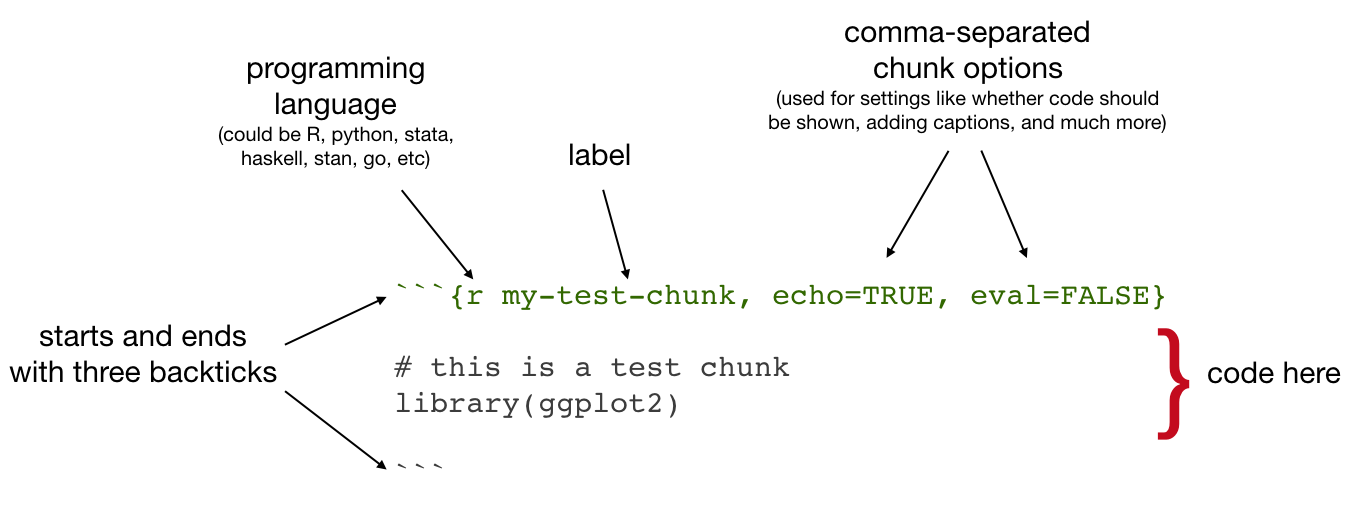
\includegraphics[width=1\linewidth]{figures/sample-content/chunk-parts} \caption{Code chunk syntax}\label{fig:chunk-parts}
\end{figure}

Common chunk options include (see e.g.
\href{https://bookdown.org/yihui/rmarkdown/r-code.html}{bookdown.org}):

\begin{itemize}
\tightlist
\item
  \texttt{echo}: whether or not to display code in knitted output
\item
  \texttt{eval}: whether or to to run the code in the chunk when
  knitting
\item
  \texttt{include}: whether to include anything from the from a code
  chunk in the output document
\item
  \texttt{fig.cap}: figure caption
\item
  \texttt{fig.scap}: short figure caption, which will be used in the
  `List of Figures' in the PDF front matter
\end{itemize}

\textbf{IMPORTANT}: Do \emph{not} use underscoores in your chunk labels
- if you do, you are likely to get an error in PDF output saying
something like ``! Package caption Error: \textbackslash{}caption
outside float''.

\subsection{Setup chunks - setup, images,
plots}\label{setup-chunks---setup-images-plots}

An R Markdown document usually begins with a chunk that is used to
\textbf{load libraries}, and to \textbf{set default chunk options} with
\texttt{knitr::opts\_chunk\$set}.

In your thesis, this will probably happen in \textbf{index.Rmd} and/or
as opening chunks in each of your chapters.

\begin{verbatim}
```{r setup, include=FALSE}
# don't show code unless we explicitly set echo = TRUE
knitr::opts_chunk$set(echo = FALSE)

library(tidyverse)
```
\end{verbatim}

\subsection{Including images}\label{including-images}

Code chunks are also used for including images, with
\texttt{include\_graphics} from the \texttt{knitr} package, as in Figure
\ref{fig:oxford-logo}

\begin{Shaded}
\begin{Highlighting}[]
\NormalTok{knitr}\OperatorTok{::}\KeywordTok{include_graphics}\NormalTok{(}\StringTok{"figures/sample-content/beltcrest.png"}\NormalTok{)}
\end{Highlighting}
\end{Shaded}

\begin{figure}

{\centering 
\includegraphics[width=0.5\linewidth]{figures/sample-content/beltcrest} 

}

\caption{Oxford logo}\label{fig:oxford-logo}
\end{figure}

Useful chunk options for figures include:

\begin{itemize}
\tightlist
\item
  \texttt{out.width} (use with a percentage) for setting the image size
\item
  if you've got an image that gets waaay to big in your output, it will
  be constrained to the page width by setting
  \texttt{out.width\ =\ "100\%"}
\end{itemize}

\subsubsection*{Figure rotation}\label{figure-rotation}
\addcontentsline{toc}{subsubsection}{Figure rotation}

You can use the chunk option \texttt{out.extra} to rotate images.

The syntax is different for LaTeX and HTML, so for ease we might start
by assigning the right string to a variable that depends on the format
you're outputting to:

\begin{Shaded}
\begin{Highlighting}[]
\ControlFlowTok{if}\NormalTok{ (knitr}\OperatorTok{::}\KeywordTok{is_latex_output}\NormalTok{())\{}
\NormalTok{  rotate180 <-}\StringTok{ "angle=180"}
\NormalTok{\} }\ControlFlowTok{else}\NormalTok{ \{}
\NormalTok{  rotate180 <-}\StringTok{ "style='transform:rotate(180deg);'"}
\NormalTok{\}}
\end{Highlighting}
\end{Shaded}

Then you can reference that variable as the value of \texttt{out.extra}
to rotate images, as in Figure \ref{fig:oxford-logo-rotated}.

\begin{figure}

{\centering 
\includegraphics[width=0.5\linewidth,angle=180]{figures/sample-content/beltcrest} 

}

\caption{Oxford logo, rotated}\label{fig:oxford-logo-rotated}
\end{figure}

\subsection{Including plots}\label{including-plots}

Similarly, code chunks are used for including dynamically generated
plots. You use ordinary code in R or other languages - Figure
\ref{fig:cars-plot} shows a plot of the \texttt{cars} dataset of
stopping distances for cars at various speeds (this dataset is built in
to \textbf{R}).

\begin{Shaded}
\begin{Highlighting}[]
\NormalTok{cars }\OperatorTok\StringTok{ }
\StringTok{  }\KeywordTok{ggplot}\NormalTok{() }\OperatorTok{+}
\StringTok{    }\KeywordTok{aes}\NormalTok{(}\DataTypeTok{x =}\NormalTok{ speed, }\DataTypeTok{y =}\NormalTok{ dist) }\OperatorTok{+}
\StringTok{    }\KeywordTok{geom_point}\NormalTok{()}
\end{Highlighting}
\end{Shaded}

\begin{figure}
\centering
\includegraphics{02-rmd-basics-markdown_files/figure-latex/cars-plot-1.pdf}
\caption{\label{fig:cars-plot}A ggplot of car stuff}
\end{figure}

Under the hood, plots are included in your document in the same way as
images - when you build the book or knit a chapter, the plot is
automatically generated from your code, saved as an image, then included
into the output document.

\subsection{Including tables}\label{including-tables}

Tables are usually included with the \texttt{kable} function from the
\texttt{knitr} package.

Table \ref{tab:cars-table} shows the first rows of that cars data - read
in your own data, then use this approach to automatically generate
tables.

\begin{Shaded}
\begin{Highlighting}[]
\NormalTok{cars }\OperatorTok\StringTok{ }
\StringTok{  }\KeywordTok{head}\NormalTok{() }\OperatorTok\StringTok{ }
\StringTok{  }\NormalTok{knitr}\OperatorTok{::}\KeywordTok{kable}\NormalTok{(}\DataTypeTok{caption =} \StringTok{"A knitr kable table"}\NormalTok{)}
\end{Highlighting}
\end{Shaded}

\begin{table}

\caption{\label{tab:cars-table}A knitr kable table}
\centering
\begin{tabular}[t]{r|r}
\hline
speed & dist\\
\hline
4 & 2\\
\hline
4 & 10\\
\hline
7 & 4\\
\hline
7 & 22\\
\hline
8 & 16\\
\hline
9 & 10\\
\hline
\end{tabular}
\end{table}

\begin{itemize}
\tightlist
\item
  Gotcha: when using
  \href{https://www.rdocumentation.org/packages/knitr/versions/1.21/topics/kable}{\texttt{kable}},
  captions are set inside the \texttt{kable} function
\item
  The \texttt{kable} package is often used with the
  \href{https://cran.r-project.org/web/packages/kableExtra/vignettes/awesome_table_in_html.html}{\texttt{kableExtra}}
  package
\end{itemize}

\subsection{Control positioning}\label{control-positioning}

One thing that may be annoying is the way \emph{R Markdown} handles
``floats'' like tables and figures. In your PDF output, LaTeX will try
to find the best place to put your object based on the text around it
and until you're really, truly done writing you should just leave it
where it lies.

In general, you should allow LaTeX to do this, but if you really
\emph{really} need a figure to be positioned where you put in the
document, then you can make LaTeX attempt to do this with the chunk
option \texttt{fig.pos="H"}, as in Figure
\ref{fig:oxford-logo-controlled}:

\begin{Shaded}
\begin{Highlighting}[]
\NormalTok{knitr}\OperatorTok{::}\KeywordTok{include_graphics}\NormalTok{(}\StringTok{"figures/sample-content/beltcrest.png"}\NormalTok{)}
\end{Highlighting}
\end{Shaded}

\begin{figure}[H]

{\centering 
\includegraphics[width=0.5\linewidth]{figures/sample-content/beltcrest} 

}

\caption{An Oxford logo that LaTeX will try to place at this position in the text}\label{fig:oxford-logo-controlled}
\end{figure}

As anyone who has tried to manually play around with the placement of
figures in a Word document knows, this can have lots of side effects
with extra spacing on other pages, etc. Therefore, it is not generally a
good idea to do this - only do it when you really need to ensure that an
image follows directly under text where you refer to it (in this
document, I needed to do this for Figure \ref{fig:latex-font-sizing} in
section \ref{max-power}). For more details, read the relevant section of
the {[}R Markdown
Cookbook{]}\url{https://bookdown.org/yihui/rmarkdown-cookbook/figure-placement.html}).

\section{Executable inline code}\label{executable-inline-code}

`Inline code' simply means inclusion of code inside text. The syntax for
doing this is \texttt{\textasciigrave{}r\ R\_CODE\textasciigrave{}} For
example, \texttt{\textasciigrave{}r\ 4\ +\ 4\textasciigrave{}} will
output 8 in your text.

You will usually use this in parts of your thesis where you report
results - read in data or results in a code chunk, store things you want
to report in a variable, then insert the value of that variable in your
text. For example, we might assign the number of rows in the
\texttt{cars} dataset to a variable:

\begin{Shaded}
\begin{Highlighting}[]
\NormalTok{num_car_observations <-}\StringTok{ }\KeywordTok{nrow}\NormalTok{(cars)}
\end{Highlighting}
\end{Shaded}

We might then write:\\
``In the \texttt{cars} dataset, we have
\texttt{\textasciigrave{}r\ num\_car\_observations\textasciigrave{}}
observations.''

Which would output:\\
``In the \texttt{cars} dataset, we have 50 observations.''

\section{Executable code in other languages than
R}\label{executable-code-in-other-languages-than-r}

If you want to use other languages than R, such as Python, Julia C++, or
SQL, see
\href{https://bookdown.org/yihui/rmarkdown-cookbook/other-languages.html}{the
relevant section of the \emph{R Markdown Cookbook}}


%%%%% REFERENCES

% JEM: Quote for the top of references (just like a chapter quote if you're using them).  Comment to skip.
% \begin{savequote}[8cm]
% The first kind of intellectual and artistic personality belongs to the hedgehogs, the second to the foxes \dots
%   \qauthor{--- Sir Isaiah Berlin \cite{berlin_hedgehog_2013}}
% \end{savequote}

\setlength{\baselineskip}{0pt} % JEM: Single-space References

{\renewcommand*\MakeUppercase[1]{#1}%
\printbibliography[heading=bibintoc,title={\bibtitle}]}

\end{document}
